\chapter{Cryptographic Sponge Functions}\label{chap:Sponge}
The SHA-2 family of functions is still considered cryptographically secure. However advances in hash function analysis threaten these crypto-systems, and as they all rely on the same underlying construction, a potential breakthrough in their cryptanalysis could break them all. Moreover selecting and implementing a new standard for all protocols that use cryptographic hashes is a slow process. This is why a new family of hash functions has been standardised: the SHA-3 family of functions, approved by the NIST in August 2015. This additional family provides resiliance against future advances in hash function analysis, as it relies on a fundamentally different design pattern: the \emph{sponge construction}.
Thus even if hash functions based on the Merkle-Damg\r{a}rd construction are broken, the SHA-3 family of functions will be at hand to replace them.

A \emph{cryptographic sponge function} is a function which uses the \emph{sponge construction} structure. This structure is defined in Section~\ref{sec:Sponge}, we then describe the standardised implementation of such sponge functions: the SHA-3\footnote{Secure Hash Algorithm-3} family.

\section{Definitions: Random Oracles, Transformations and Permutations}
We denote a random oracle by $\mathcal{RO}$.
\begin{defn} A random oracle $\mathcal{RO}$ takes as input binary strings of any length and returns for each input a random infinite string, i.e., it is a map from $\mathbb{Z}_2^∗$ to $\mathbb{Z}_2^{\infty}$, chosen by selecting each bit of $\mathcal{RO}(M)$ uniformly and independently, for every $M$.
\end{defn}
A $\mathcal{RO}$ whose output is truncated to its $l$ first bits is denoted $Z = \mathcal{RO}(M, l)$. 
We also need the concept of a random (fixed-width) transformation.
\begin{defn} A \emph{random transformation} with given width $b$ is a transformation drawn randomly and uniformly from the set of all $2^{b\cdot 2^b}$ b-bit transformations.
\end{defn}
Finally, we define a random (fixed-width) permutation.
\begin{defn} A \emph{random permutation} with given width $b$ is a permutation drawn randomly and uniformly from the set of all $2^b\!$ b-bit permutations.
\end{defn}

\section{Construction}\label{sec:Sponge}
\subsection{Outline}
The sponge construction is a simple iterated construction for building a function F with \emph{variable-length input and arbitrary output length} based on a \textbf{fixed-length transformation or permutation $f$} operating on a fixed number $b$ of bits. Here $b$ is called \textbf{the width}.

The sponge construction operates on a state of $b = r + c$ bits. The value $r$ is called \textbf{the bitrate} and the value \textbf{$c$ the capacity}.

First, all the bits of the state are initialized to zero. The input message is padded and cut into blocks of $r$ bits. 

The sponge construction then proceeds in two phases: the absorbing phase, during which all message blocks are processed, followed by the squeezing phase, which outputs the number of output blocks chosen by the user.


\subsection{The Sponge Construction}\label{section:sponge}
The sponge construction builds a function \textsc{sponge}[$f$,pad,r]: $\mathbb{Z}_2^∗ \rightarrow \mathbb{Z}_2^\infty$ using:
\begin{itemize}[label=\textperiodcentered,nolistsep]
\item a fixed-length transformation or permutation $f{\{0,1\}}^b \rightarrow {\{0,1\}}^b$
\item a sponge-compliant padding rule “pad”
\item and a parameter \textbf{bitrate} $r$.
\end{itemize}
A finite-length output can be obtained by truncating it to its $l$ first bits. We call an instance of the sponge construction a \textbf{sponge function}.

The transformation or permutation $f$ operates on a fixed number of bits, the \textbf{width $b$}. The sponge construction has a \textbf{state} of $b$ bits. 

First, all the bits of the state are initialized to zero. The input message is padded and cut into $r$-bits blocks. Then it proceeds in two phases: the \emph{absorbing phase} followed by the \emph{squeezing phase}. During both these phases we distinguish the first $r$ bits of the state, called the \textbf{outer part} and denoted \textbf{$\overline{s}$}, from the remaining $b − r$ bits of the stated, called the \textbf{inner state $\widehat{s}$}. These two parts of the state will be treated differently by the sponge construction.  The inner state is of length $b − r$ and is called the \textbf{capacity c}. 

The two phases are:
\begin{itemize}
\item \textbf{Absorbing phase}: The $r$-bit input message blocks are XORed into the outer part $\overline{s}$ of the state, interleaved with applications of the function $f$. When all message blocks are processed, the sponge construction switches to the squeezing phase.

\item \textbf{Squeezing phase}: The outer part of the state is iteratively returned as output blocks, inter-leaved with applications of the function $f$. The number of iterations is determined by the desired number of bits $l$.
\end{itemize}

Finally the output is truncated to its first $l$ bits. The $c$-bit inner state is never directly affected by the input blocks and never output during the squeezing phase. The capacity $c$ actually determines the attainable security level of the construction. We use the term \emph{random sponge} to denote a sponge function with $f$ a random transformation or permutation.

The sponge construction is illustrated in Figure~\ref{fig:sponge}, and Algorithm~\ref{algo:sponge} provides a formal definition.

In this representation the state is a binary string of a given length $b$ and the message blocks are $r$-bit strings.

\begin{figure}[H]
\centering
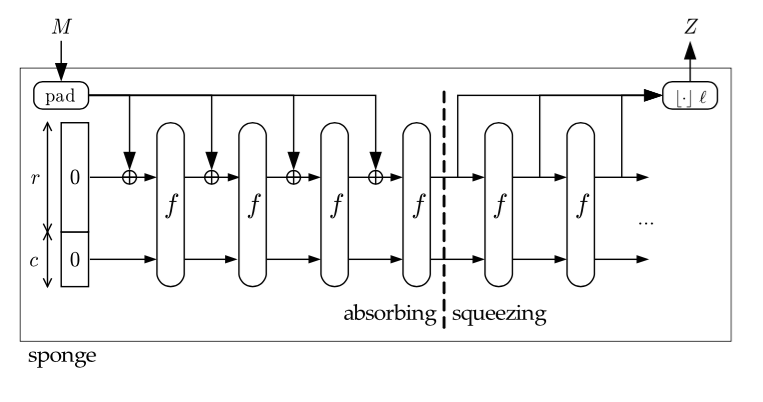
\includegraphics[scale=0.5]{img/sponge1.png}
\caption{\label{fig:sponge}The sponge construction $Z = \textsc{sponge}\lbrack f , pad, r\rbrack (M, l)$}
\end{figure}


\begin{algorithm}[H]
\caption{The sponge construction \textsc{sponge}[f, pad, r] (M,l)}
\label{algo:sponge}

\begin{algorithmic}[1]
\Require{$r < b$}

\Ensure{$Z = sponge(M, l)$ with $M \in \mathbb{Z}_2^∗$, $l \in \mathbb{N}^{*+}$ and $Z ∈ \mathbb{Z}_2^l$}

\State{$P = M\vert \vert pad\lbrack r\rbrack (\vert M\vert )$ }
\State{$s = 0^b$}

\For{$i \gets 0$ to $\vert P\vert_r − 1$ }
\State{$s = s \oplus (P_i\vert \vert0^{b−r})$}
\State{$s = f(s)$}
\EndFor{}

\State{$Z = \lfloor s\rfloor_r$}

\While{$\vert Z\vert_r \times r < l$}
\State{$s = f(s)$}
\State{$Z = Z\vert \vert \lfloor s\rfloor _r$ }
\EndWhile{}

\Return{$\lfloor Z\rfloor _l$}
\end{algorithmic}
\end{algorithm}


\subsection{Auxiliary Functions}\label{section:aux}
In this section we introduce two additional functions \textsc{absorb} and \textsc{squeeze} which represent the two phases of the sponge function introduced above. These will help in the understanding of attacks on the sponge function.


The absorbing function \textsc{absorb}[f, r] takes as input a string $P$ with $\vert P\vert$ multiple of $r$ and returns the value of the state after absorbing P. The absorbing function is defined in Algorithm~\ref{algo:absorb}.

\begin{algorithm}[H]
\caption{The absorbing function \textsc{absorb}[f, r]}
\label{algo:absorb}
\begin{algorithmic}[1]
\Require{$r < b$}
\Ensure{$s=absorb(P)$ with $P \in \mathbb{Z}_2^∗$ and $s \in \mathbb{Z}_2^b$}

\State{$s = 0^b$}

\For{$i = 0$ to $\vert P\vert_r − 1$}
\State{$s = s \oplus (P_i\vert \vert0^{b−r})$}
\State{$s = f(s)$ }
\EndFor{}

\Return{$s$}
\end{algorithmic}
\end{algorithm}

The squeezing function \textsc{squeeze}[f, r] takes as input a state $s$ and a positive integer $l$. This function returns the output truncated to $l$ bits of the sponge function with $s$ the state at the beginning of the squeezing phase. The squeezing function is defined in Algorithm~\ref{algo:squeeze}.

\begin{algorithm}[H]
\caption{The squeezing function \textsc{squeeze}[f, r]}
\label{algo:squeeze}

\begin{algorithmic}[1]
\Require{$r < b$}

\Ensure{$Z=squeeze(s,l)$ with $s \in \mathbb{Z}_2^b$, $l \in \mathbb{N}^{*+}$ and $Z \in \mathbb{Z}_2^l$}

\State{$Z = \lfloor s\rfloor_r$}


\While{$\vert Z\vert_r \times r< l$}
\State{$s = f(s)$}
\State{$Z = Z\vert \vert \lfloor s\rfloor _r$ }
\EndWhile{}

\Return{$\lfloor Z\rfloor _l$}

\end{algorithmic}
\end{algorithm}


\begin{defn}
$P$ is a \emph{path to the state} $s$ if $s = absorb(P)$.
\end{defn}

Clearly \textsc{absorb}[f, r]$($empty string$) = 0^b$. In general, the $j$-th block of the output of a sponge function corresponding to an input $M$ is equal to:
\begin{equation}
Z_j = \overline{\textsc{absorb}[f, r]}(P\vert \vert 0^{rj})\mbox{, } j \ge 0,
\end{equation}
with $P = M\vert \vert pad\lbrack r\rbrack (\vert M\vert)$.

Indeed, the for loop of \textsc{absorb}[f, r] will be ran $\vert P\vert_r +1$ times to $P\vert \vert 0^{rj}$. However for the last $j$ iterations of the loop, the \textsc{xor}ing of the input message blocs with the state will have no effect, as for $i\ge \vert P\vert_r$, $M_i=0^r$. Thus each iteration for $i\ge \vert P\vert_r$ only applies $f$  to the state, which is what the squeezing phase does.

Alternatively, the absorbing function can be used to express the states that the sponge traverses both as it absorbs an input M and as it is being squeezed. The traversed states are $absorb(P')$ for any $P'$ prefix of $P\vert \vert 0^\infty$, with $P = M\vert \vert pad\lbrack r\rbrack (\vert M\vert )$, including the empty string.

\subsection{Generic Primary Attacks On A Sponge Function}

The attacks hereby described are \emph{generic attacks}. For sponge functions we define it as follows: 

\begin{defn}
An attack on a sponge function is a generic attack if it does not exploit specific properties of $f$.
\end{defn}

We call \emph{primary attacks}, attacks that would not apply to $\mathcal{RO}$'s as they have no concept of state, but will apply to sponge functions due to their finite state.

These concepts are fundamental as they introduce upper-bounds to the security of any real sponge function.

As seen previously, the sponge function can be seen as the subsequent application of a padding rule, the \textsc{absorb} function and the \textsc{squeeze} function.

\begin{nota}
If $Z=$\textsc{sponge}$\lbrack f$, pad,$r\rbrack(M,l)$, we call:
\begin{equation}
\begin{aligned}
P & = M\vert \vert pad \lbrack r \rbrack (\vert M \vert )  \\
s & = \mbox{\textsc{absorb}} \lbrack f,r \rbrack (P) \\
Z & = \mbox{\textsc{squeeze}} \lbrack f,r \rbrack (s,l) \\
\end{aligned}
\end{equation}
\end{nota}
Let us consider the cryptographic requirements of a hashing function:
\subsubsection{Cryptographic resistance of the absorb function}
It is in general difficult to find a pre-image to either of the auxiliary functions introduced in Section~\ref{section:aux} i.e.\ it is difficult to find a path $P$ to a given state $s$, and it is difficult to find the state $s$ for a given output $Z$.

\begin{defn}
A \emph{state collision} is a pair of different paths $P \ne Q$ to the same state: \textsc{absorb} ($P$) = \textsc{absorb} ($Q$).
\end{defn}
It is generally hard to find two paths leading to the same state. It is therefore also difficult to find a pre-image to the \textsc{absorb} function i.e.\ it is difficult to find a path $P$ to a given state $s$.

\paragraph{Consequences of state collision}
If a state collision is obtained during the absorbing phase, an overall collision for the sponge function is easily obtainable.
If \textsc{absorb} ($P$) = \textsc{absorb} ($Q$) then the squeezing part will produce the same output values for \textsc{absorb} ($P\vert \vert 0^{rj}$) = \textsc{absorb} ($Q\vert \vert 0^{rj}$) for all j.

A state collision can also lead to a periodical output if $\exists d$ such that \textsc{absorb} ($P$) = \textsc{absorb} ($P\vert \vert 0^{rd}$). The periodicity would then be of $d$ output blocks (since $s_{\vert M\vert_r + j} = \textsc{absorb}(P\vert \vert 0^{rj})$).


\begin{defn}
An \emph{inner collision} is a pair of different paths $P \ne Q$ to the same inner state:
$\widehat{\textsc{absorb}}(P) = \widehat{\textsc{absorb}}(Q)$.
\end{defn}

Clearly a state collision implies an inner collision, and as explained below, a state collision can easily be obtained from an inner collision.

If we have an inner collision $\widehat{\textsc{absorb}}(P) = \widehat{\textsc{absorb}}(Q)$, then for any $A,B \in \mathbb Z_2^r$ that verify $\overline{\textsc{absorb}}(P)\oplus A = \overline{\textsc{absorb}}(Q) \oplus B$, the paths $P\vert \vert A$ and $Q \vert \vert B$ will lead to a state collision.

\subsubsection{Cryptographic resistance of the squeeze function}
In general it is hard to find a state s such that $\textsc{squeeze}(s, \vert Z\vert ) = Z$ for long strings Z. Depending on the origin of Z and the goal of the adversary, we distinguish two cases: 
\begin{itemize}[label=\textperiodcentered,nolistsep]
\item \emph{output binding}: Z is not necessarily the result of the squeezing of the state and so there may be no solution.
\item \emph{state recovery}: Z has been obtained by the squeezing of a state s.
\end{itemize}
Let us define these two problems formally:
\begin{defn}
Given an arbitrary string Z, \emph{output binding} is finding a state s such that $\textsc{squeeze}(s, \vert Z\vert ) = Z$.
\end{defn}
The expected number of states that squeeze to a given string $Z$ is $2^{b−\vert Z\vert}$. If $\vert Z\vert  > b$, the probability that such a state exists is $\approx 2^{b−\vert Z\vert }$.

\begin{defn}
State recovery is finding a state s, given a string Z with $Z = \textsc{squeeze}(s, \vert Z\vert )$.
\end{defn}


If $\vert Z\vert > b$, it is likely that there is only a single solution and that output binding results in recovery of the unique state that it was squeezed from. If $\vert Z \vert \le b$ there are typically several states that squeeze to $Z$ and output binding does not necessarily result in state recovery.
